\chapter{Design}

In this section, the benchmark problem will be defined and mapped as DCOP, the framework design will be explained and the mapping of the algorithms on to the Signal/Collect framework will be described. Additionally, the design and considerations regarding the monitoring platform will be presented.

\section{Meeting Scheduling Problem}

\subsection{Formal Definition as DCOP}

The formulation of the meeting scheduling problem follows the basic definition of a distributed constraint optimization problem. Agents, variables and their relationships, as well as constraints shall be formulated. The components of a meeting scheduling problem are participants, their schedule, meetings and a given timeframe. For the sake of simplicity, it was decided to not take travel time between meetings or other parameters into consideration as certain researchers have done. It was also decided to use utilities instead of costs. % FIXME find zitat

\theoremstyle{hardconstraint2}
\newtheorem{hardconstraint2}{Definition}
\begin{hardconstraint2}
Participant - has preferences and meeting he/she need to attend
\end{hardconstraint2}
\begin{hardconstraint2}
Meeting - has participants and needs to be held at an agreable time
\end{hardconstraint2}

%-------------------------- Variable  & Agent definition ------------------------------------------------
\begin{figure}[h!]
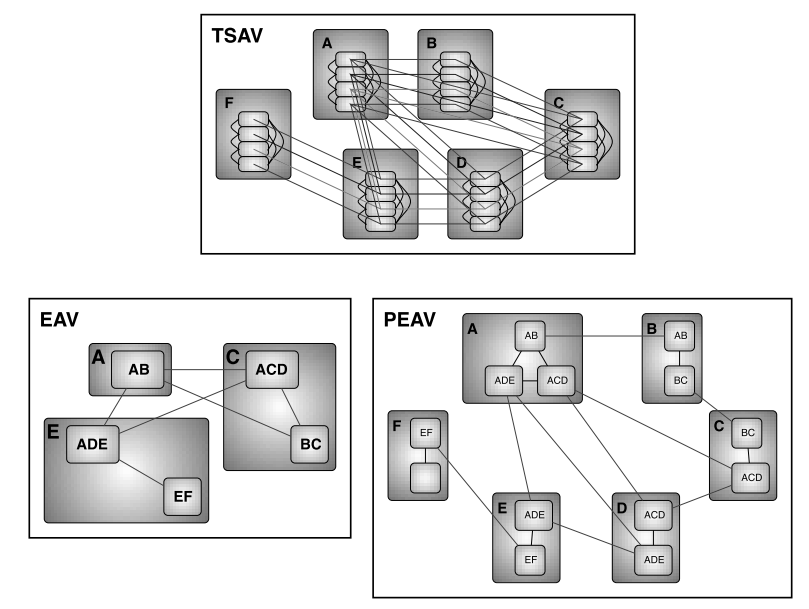
\includegraphics[width=300px]{graphics/variablemodell.png}
\caption{Different paradigms of mapping the meeting scheduling Problem \cite{Maheswarana}.}
\label{fig:variablemapping}
\end{figure}
\cite{Maheswarana} propose three different ways of mapping a meeting scheduling problem to variables (Figure \ref{fig:variablemapping}). TSAV (Time Slots As Variables), EAV (Event As Variables) and PEAV (Private Events As Variables). In EAV, every participant holds a private variable containing the preference value for a specific event. PEAV is a modification of the EAV paradigm where agents do not share their local valuations. It was decided to follow the PEAV principle and model every meeting participation of an agent as one variable instead of using timeslots as variables. An agent therefore can hold multiple variables. This paradigm has also been tried by other researchers, which further established confidence in the decision \cite{Petcu2003}.
\begin{hardconstraint2}
Agent - holds one variable per meeting participation
\end{hardconstraint2}
\begin{hardconstraint2}
Variable - represents one meeting participation
\end{hardconstraint2}
%---------------------------- Domain & Value  definition -----------------------------------------------
A variable takes on a value \(s_{i} \in S_{i}\) in a defined problem domain \(D_{i}\). In the formulation of the meeting scheduling problem, the domain represents a finite set of timeslots and the variable assigns to one of these timeslots. This value represents the currently locally chosen timeslot for a specific meeting.
\begin{hardconstraint2}
Domain - holds a finite set of possible timeslots to schedule a meeting
\end{hardconstraint2}
\begin{hardconstraint2}
Value - assignment to a timeslot of the available timeslots in the Domain
\end{hardconstraint2}
%------------------------------ Constraints ---------------------------------------------------
From the problem definition in chapter 2, one can derive soft and hard constraint for the meeting scheduling problem. Soft constraints can possibly be constructed from the preferences of the participants and utilized to maximize the utility \cite{Franzin}. Three differently weighted soft constraints have been defined to model preferences of agents. Preferred timeslots gain the highest utility, followed by free timeslots and blocked timeslots, which gain no value at all. Further, a timeliness soft constraint was defined that adds a higher utility to earlier timeslots. All of the soft constraints have unary relationships, i.e. are local. % FIXME \cite{Chapman2011} \cite{chun, andy 2003}\cite{mes, martijn 2007}\cite{BenHassine2007}\cite{Berger2008}
Additionally, two hard constraints with k-ary relationships to variable neighbours need to be formulated. The first would be an equality constraint on the assigned timeslot value for a specific meeting between all variables related to this meeting. The second is a difference constraint of assigned values between all variables of an agent \cite{Farinelli} \cite{Scheduling}.
A local utility function \(u_{l}(s)\) would therefore include the sum of all soft constraints multiplied by the product of the hard constraints analogous to the global function defined in chapter {\ref{chap:background}}. 
\[ u_{l}(s) = \prod_{\substack{hc_{k} \in HC}} u_{SC_{g}}(s) \bigg( \sum_{sc_{k} \in SC} u_{SC_{g}}(s) \bigg)\] 

%---------------------------- Conclusion from this ----------------------------------
The conclusions from this formal definition in regards to the general structure of the algorithms is to have one variable represent each meeting participation of an agent. The agent is therefore an abstract definition of a set of meeting participation nodes. All variables of an agent should share a reference to an integrating agent vector, where meeting times are registered. This agent vector acts as a difference hard constraint between the different meeting participations of an agent. Further, all variables attending a meeting also share a reference to the meeting vector where every agent shares his current preference. This represents the aforementioned equality hard constraint. It was further decided to implement the given local utility function in the framework as a generalized method, as the structure repeats itself in all thre algorithms and because it is further helpful for comparison to have the exact same utility function implemented.

\subsection{Problem Dataset Generation}

% ------------------------ Entscheidung, Verteidigung --------------------
During the course of the thesis, it was necessary to find a dataset for the benchmarking. The Frodo2\footnote{http://frodo2.sourceforge.net} framework or for example the dataset from AAMAS 2004 \footnote{http://teamcore.usc.edu/dcop/} do provide a couple of datasets for meeting scheduling. But because it was considered that in the benchmarks one would need to be able to produce problems with different densities and scale to high numbers of participants, as well as change constraints dynamically it was decided to generate meeting participations and agent schedules randomly. It was also chosen to limit the number of meeting participations per agent to keep the benchmarks more realistic analogously to \cite{Chun2003}.

\begin{itemize}
\item The blocked timeslots in a schedule are based on the percentage given trough the density parameter
\item Preferences for meetings are chosen randomly from free timeslots in the schedule
\item The number of meeting participations is chosen randomly from 1-5
\item The meeting participations are chosen at random
\end{itemize}

\section{Framework}

\subsection{Signal / Collect}
The foundation of the implementations in this thesis is the Signal/Collect framework\footnote{http://uzh.github.io/signal-collect} \cite{Stutz2010}, which is built on top of Akka\footnote{http://akka.io} and written in Scala\footnote{http://www.scala-lang.org}. It is a graph processing engine with a programming paradigm comparable to Map/Reduce \cite{Dean2008}. The main components are vertices and edges, as well as a graph structure where those components are added. A vertex has a state and sends signals along it's edges to connected vertices, which can contain any datatype. The signal usually is the state of the vertex or calculated in context of it. Vertices gather the signals of connected nodes and run the defined collect function on the received information. The state of a vertex is usually adjusted according to the results of these calculations and the next signal that is sent will include this state.  This model allows to reduce complex algorithms to a few lines of code and is applicable for many problems. The framework further has the capability of running graph processings asynchronously or with synchronous signal steps and it is possible to distribute the system on multiple machines. Reasons for choosing this framework are the excellent structural fit for distributed constraint optimization problems, synchronous and asynchronous run modes and the possiblity to add and remove vertices during run-time as it allows for dynamically changing problems.

\subsection{Structure \& Functionality}
A specific framework for benchmarking dynamic problems has been implemented. It was considered that the basic structure of the framework should help with the control of the benchmark runs and add the general ability to change a problem during runtime. This functionality was designed as problem agnostic and abstracted. The main hierarchy in the framework is the vertex stack. A \texttt{BasicVertex} has been implement containing a basic convergence function and control parameters related to the number of signal steps. Further, a \texttt{MeetingSchedulingVertex} has been implemented. This vertex implements all generalizable functions of the three benchmark algorithms described in chapter 3.1. A main component is the handling of the agent vector and the meeting vectors, a convergence function for meeting scheduling, the local utility function and data storage functions. 
To generalize dynamic change functions, a \texttt{DynamicVertex} has been created, which implements methods for changing constraints and the value domain of the vertex. The specific vertex implementations of the three implement DCOP algorithms extend the \texttt{DynamicVertex}.
\newline \newline
The initial design consideration to introduce change to the constraints of the agents has been to create a special vertex as part of the graph in Signal/Collect as the framework supports multiple types of vertices and messages in one graph execution. However, the vertex needed to be paused in the case of interval changes for a certain time and this caused errors during execution. Akka distributes multiple actors to the same thread and through pausing the \texttt{DynamicVertex}, other vertices were blocked. It therefore was decided to run the change controller in a separate thread alongside the graph execution. The main ability of the controller is to change constraints at a given interval and percentage (of all constraints in the problem). This allows testing of the stability of the algorithms. It is further possible to run a single change after a given interval. In the case of the meeting scheduling problem implementation this is only related to soft constraints as hard constraints can be handled by adding or removing variables with the second function. The controller also implements a variable change function, which similarily can be run at a certain interval or at one timepoint.  One can add parameters to create a new neighbourhood or use existing relationships and add new variables or remove existing vertices. Instead of being defined by percentage, this change is given by number. As a third function, the controller does change the domain in the whole problem for all agents. In the use case of meeting scheduling, this increases or reduces the available timeslots.
\newline \newline
The parameters and run modes of the framework have been designed with the benchmarks of this thesis in mind.  It is possible to pass general run parameters for algorithm type, for Signal/Collect run mode (synchronous/asynchronous) and one can specify to the software to run in normal mode or in one of the dynamic change variations (\texttt{changeConstraints}, \texttt{changeVariable}, \texttt{changeDomain)} with specific parameters.  It is further possible to add meeting scheduling specific parameters. For this thesis, the parameters for problem density (blocked timeslots percentage), timeslots, number of meetings and number of meeting participants were defined. For testing purposes, it is possible to start the framework via SingleTest or MultiTest. SingleTest runs one setting once and MultiTest allows to specifiy a range and scale of agents and meetings that should be tested.

\subsection{Monitoring Platform}
The  storage and monitoring of the utilities, quality levels, conflicts and run statistics of the calculations is usually done by writing the results to a log file. It was decided to use an alternative method during the course of this thesis. Mainly because it was a desirable function  to automatically post-process the results of the bechmarks on a detached machine and because real-time visibility was considered to be useful during the implementation of the algorithms.\newline Sending the results with non-blocking asynchronous HTTP requests\footnote{http://dispatch.databinder.net} to a restful API on a dedicated server was considered to be a viable option and worth trying out. The Play Framework\footnote{https://www.playframework.com} has been chosen for implementation because it is highly scalable and able to handle thousands of simultanous connections, is lightweight as well as non-blocking and allows to process results on-the-fly with code written in Java or Scala. It was also chosen because the Akka framework, which is also the foundation of Signal/Collect is tightly integrated and the actors concept is an integral part of the platform. For every benchmarking run, an actor is created that handles all the relevant incoming messages. It is therefore possible to run multiple benchmarks in parallel. The framework further allows to visualize the global utility of the graph in real-time via websockets.

\begin{figure}[H]
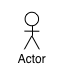
\includegraphics[width=300px]{graphics/monitoring}
\centering
\caption{The real-time view of the Monitoring Platform}
\label{fig:monitoring}
\end{figure}

\section{Mapping of DPOP}

The following sections describes the mapping of the graph structure of the DPOP algorithm and the behaviour of it's nodes described in chapter 2.3.1 to the Signal/Collect Framework  in regards to the meeting scheduling problem. The implementation is based on \cite{Petcu2003}.

\subsection{Graph Structure}
\begin{figure}[h]
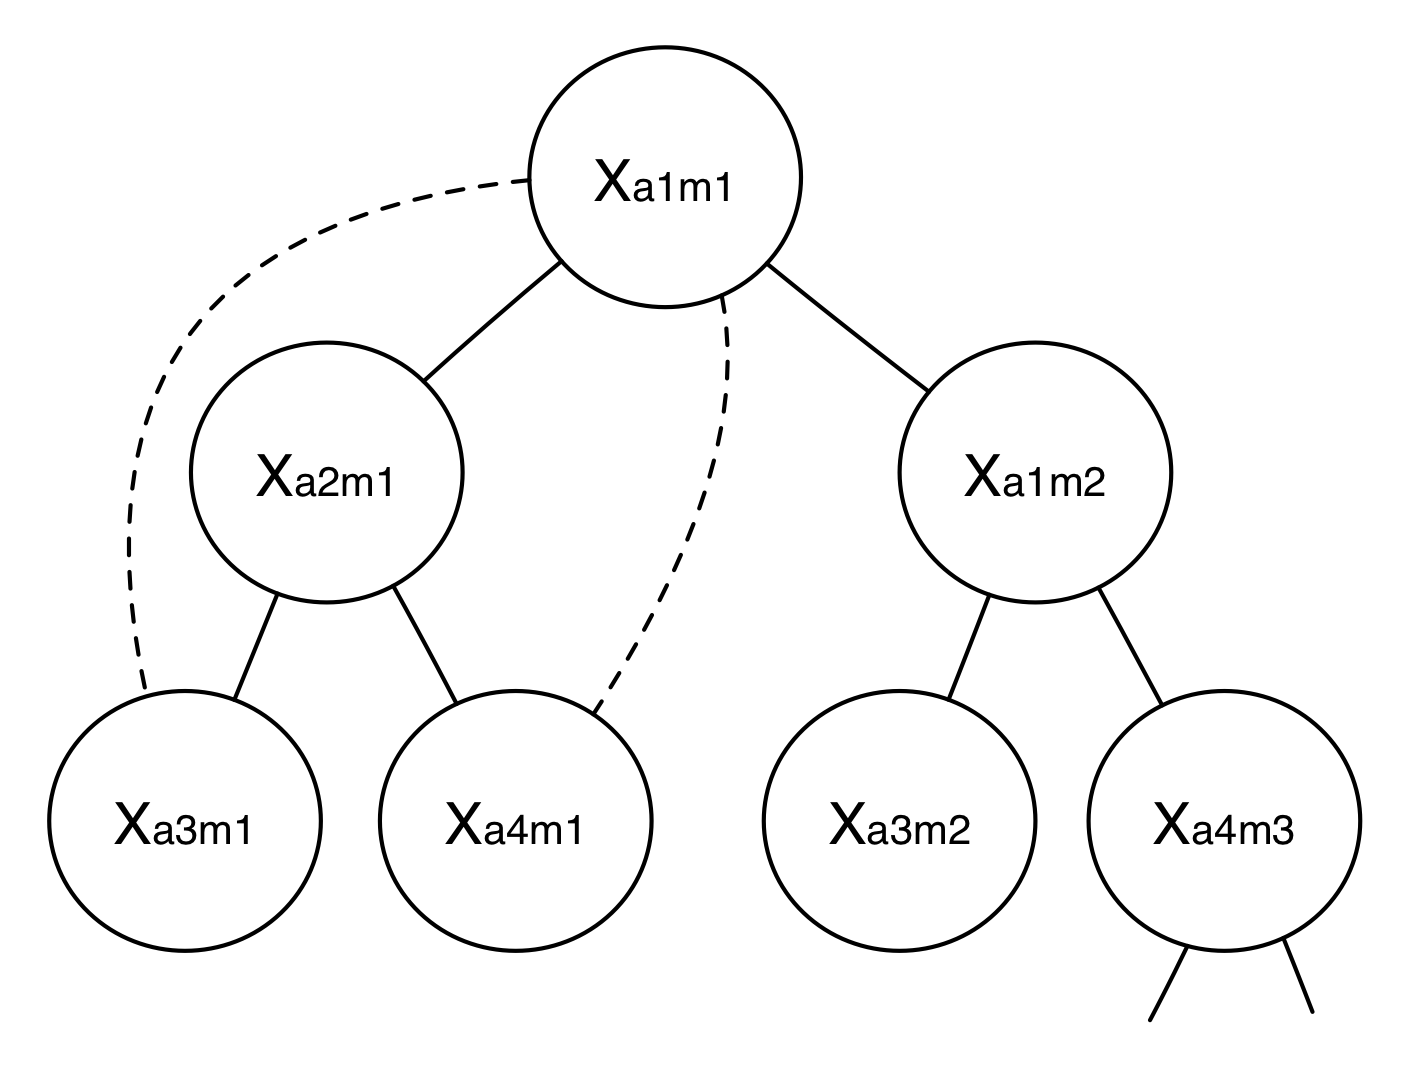
\includegraphics[width=200px]{graphics/dpop_graph}
\centering
\caption{An example DPOP pseudotree}
\label{fig:dpop_graph}
\end{figure}

Following the definition of \cite{Petcu2003} and the descriptions in chapter 2.3.1, the graph was arranged as a pseudotree. As mentioned in chapter 3.1.1, every agent is represented through meeting participation nodes as a general rule for the algorithm implementation. To create a pseudotree, one needs to transform an existing graph. Therefore, a graph has been constructed where all meeting participation vertices that share the same meeting are connected with edges. The chosen implementations of Signal/Collect components for the graph are the \texttt{DataGraphVertex} and the \texttt{StateForwarderEdge} classes. After the inital graph is created it is transformed to a pseudotree, which is a root tree with binary parent-child relationships that contains the same vertices as the original graph. An important attribute is that previously connected vertices are put into the same branch \cite{Petcu2003}. As one can see in Figure \ref{fig:dpop_graph}, the original participants have been put into the tree according to this rule. The visible participant of meeting three is inserted into the tree at a lower level than the vertices of meeting one and two, but does also hold this property. The original edge connections remain as so-called back-edges (dashed line) and the new connections are also implemented as Signal/Collect edges (solid line). This tree arrangement leads to cycles. The vertices of the same agent share an agent vector, which is not visualized in Figure \ref{fig:dpop_graph}.

\subsection{Vertex Functions}
In DPOP, a node does receive util messages from it's children and value messages from the parent vertex in the graph. These messages have been implemented as a \texttt{DPOPMessage} signal object that either is a util or a value message. The collect function of a vertex does decide from whom the message has been received and stores them in their respective vector. The following util propagation and value propagation phases and the calculations of their respective handler functions are defined by the position of the vertex in the tree.
\newline \newline
\begin{algorithm}[H]
 \TitleOfAlgo{Max-sum (node n)}
 \KwFunctions{Util Message Handler Uxk, Utilxk(xi)}
 Store util xk(xi)\;
       \Ife{} {
           \;
        }
       {
           \;
        }
    }
    return\;
 \caption{DPOP Util Message Handler \cite{Petcu2003}}
 \label{alg:dpop_util}
\end{algorithm}
A leaf node always does compute its utilities in the util propagation phase as it does not receive any util messages. In the case of the meeting scheduling problem, utilities for every timeslot are being calculated. If the vertex is the root of the tree it does only receive util messages. Those include the combined utilities of all nodes along the path to the top. The vertex then chooses the optimal timeslot value for every meeting. If the node is in the middle, it does receive both types of messages. Such a vertex computes the combined utilities from the received utility messages and it's own utilities during the util propagation phase (Algorithm \ref{alg:dpop_util}). 
\newline \newline
%\begin{algorithm}[H]
% \KwFunctions{Util Message Handler Uxk, Utilxk(xi)}
% Store util xk(xi)\;
%       \Ife{} {
%           \;
%        }
%       {
%           \;
%        }
%     send $\(m_{n'}\)$ to $\(n'\)$\;
%    }
%    return\;
% }
% \caption{DPOP Value Handler \cite{Petcu2003}}
% \label{alg:dpop_value}
%\end{algorithm}
%\newline \newline
In the value propagation phase, all received values are combined by the vertices and an optimal value for the vertex specific meeting is chosen locally (Algorithm \ref{alg:dpop_value}}). In the implementation, the util propagation phase and the value propagation phase are calculated successively and the resulting utilites and values are stored in a\texttt{DPOPMessage}. The message is then sent to all connected vertices.

\section{Mapping of MGM}

The following section describes the mapping of the graph structure of the Maximum-Gain Messaging algorithm and the behaviour of it's nodes described in chapter 2.3.2 to the Signal/Collect Framework in regards to the meeting scheduling problem. The implementation is based on \cite{Chapman2010}.

\subsection{Graph Structure}
\begin{figure}[H]
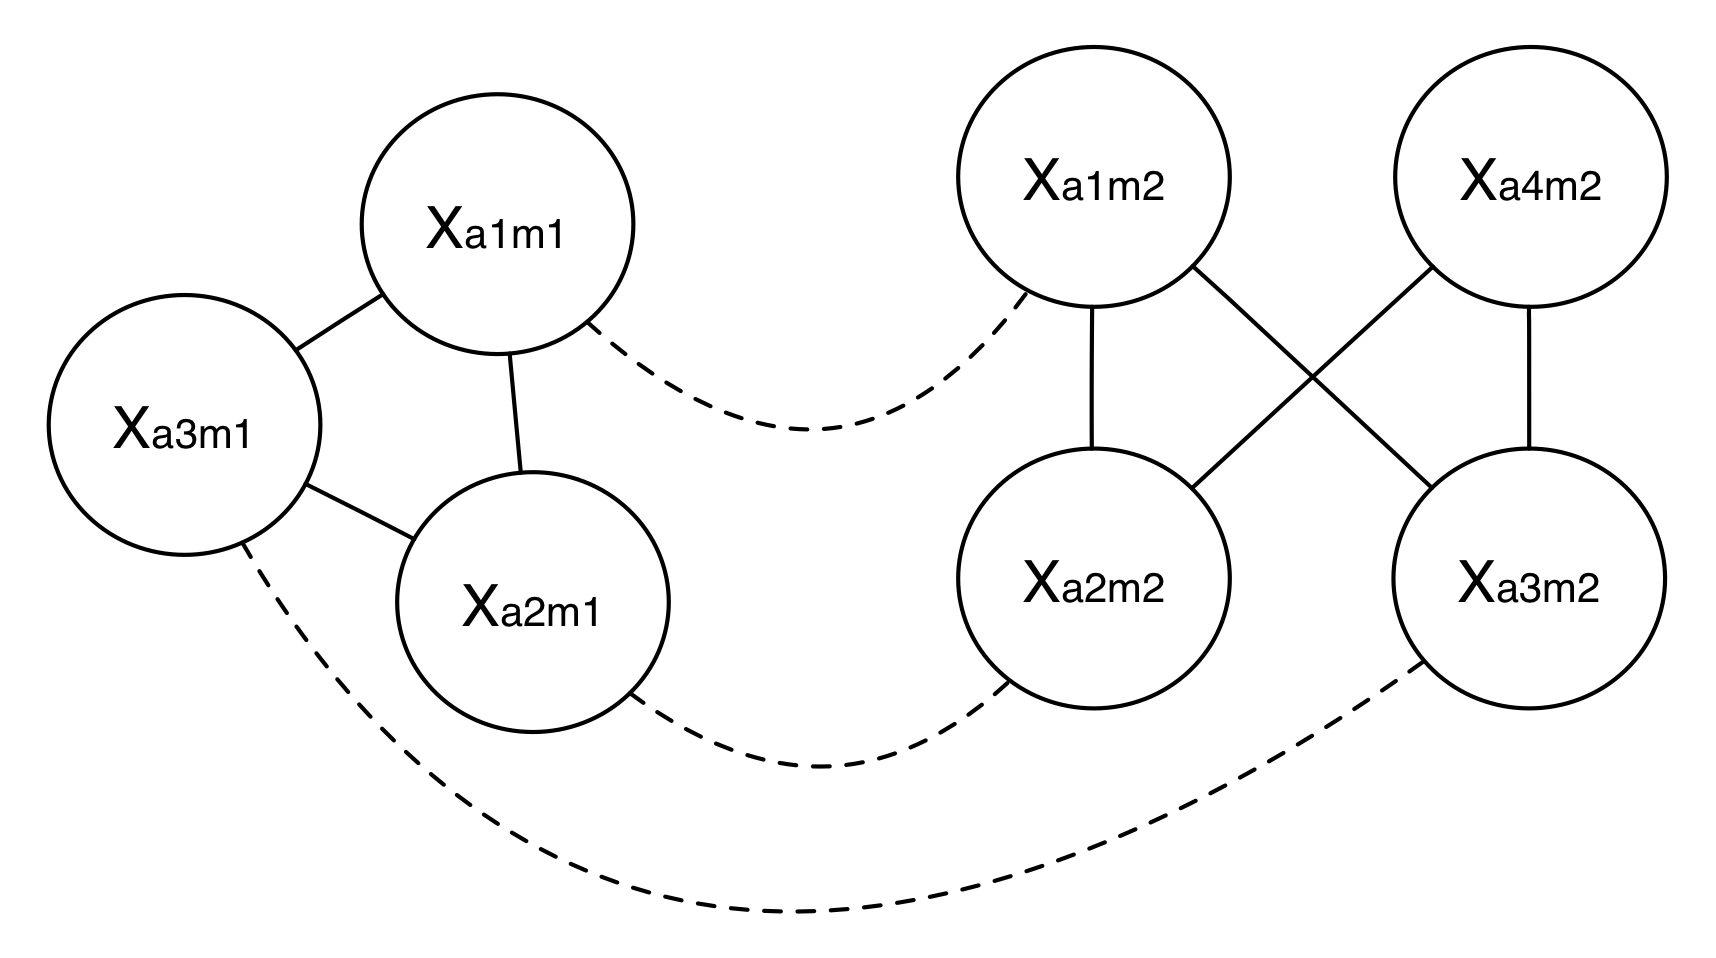
\includegraphics[width=250px]{graphics/mgm_graph}
\centering
\caption{An example MGM graph}
\label{fig:mgm_graph}
\end{figure}

Mapping the meeting scheduling problem to the structure of the MGM algorithm was quite straightforward. The participant vertices of one meeting are all connected to each other through a Signal / Collect edge comparable to the initial graph setup in the DPOP implementation. The vertices have been implemented with the \texttt{DataGraphVertex} as base class and the edges are of the class \texttt{StateForwarderEdge}. As one can see in Figure \ref{fig:mgm_graph}, the vertices of the same agent are created with a reference to the same agent vector (dashed line) and therefore to each other. This connection is virtual and not implemented as Signal/Collect edge (solid line) in the graph.

\subsection{Vertex Functions}
In MGM there are also two types of messages. A gain message and a value message. Similar to the implementation of DPOP, a \texttt{MGMMessage} has been implemented, which can be both and is interpreted by the collect function as the respective type. Initially, a local best-gain is generated by comparing the utility increase from the initaly random meeting timeslot preference to the possible timeslot with the highest utility. This best-gain value is sent to the neighbours.  If a vertex has received gain messages, it does compare them to the last local best-gain value and determines if one message contains a higher gain value. If the local gain is still the highest, the vertex converges to the value that delivers this gain. A message with the local state, i.e. the meeting preference is sent to the other vertices. If the vertex does not have the highest gain, it does continue by sending its gain value again. 
\newline \newline
\begin{algorithm}[H]
 \TitleOfAlgo{Max-sum (node n)}
 $\(N_{n}\) \leftarrow$ all of $\(n\)$'s neighboring nodes\;
 \While{no termination condition is met}{
  collect messages from $\(N_{n}\)$\;
  \ForEach{$\(n' \in N_{n}\)$}{
       \If{$\(n\)$ is a variable-node} {
           produce message $\(m_{n'}\)$ using messages from $\(N_{n} \setminus \{n'\}\)$\;
        }
       \If{$\(n\)$ is a function-node} {
           produce message $\(m_{n'}\)$ using constraint and messages from $\(N_{n} \setminus \{n'\}\)$\;
        }
     send $\(m_{n'}\)$ to $\(n'\)$\;
    }
 }
 \caption{MGM Pseudocode \cite{Chapman2010}}
 \label{alg:mgm}
\end{algorithm}

\section{Mapping of MaxSum}

The following sections describe the mapping of the graph structure of  and the behaviour of it's nodes described in chapter 2.3.3 to the Signal/Collect Framework  in regards to the meeting scheduling problem. 

\subsection{Graph Structure}

\begin{figure}[H]
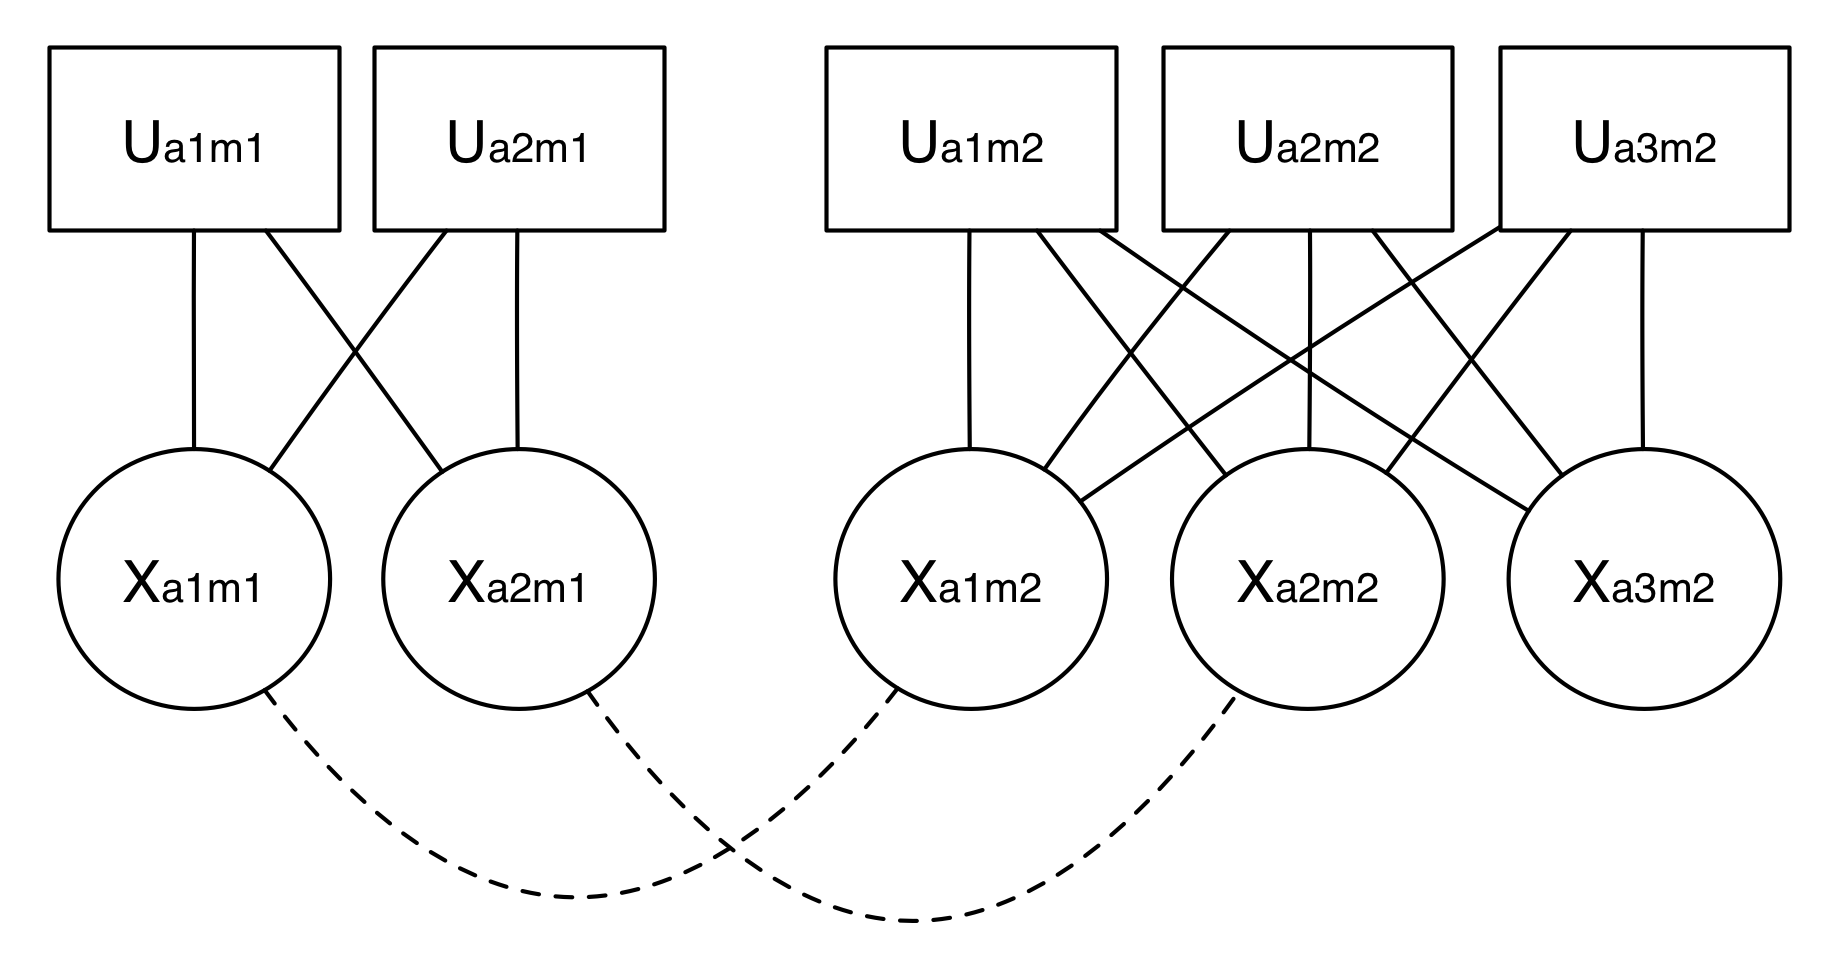
\includegraphics[width=250px]{graphics/maxsum_graph}
\centering
\caption{An example MaxSum graph}
\label{fig:maxsum_graph}
\end{figure}

A MaxSum graph is a tranformation of a common DCOP graph to a factor graph, where each variable has an additional function node attached. This function node represents a constraint and is connected to the previous neighbours. The variable node is connected to the function node of it's previous neighbours. Mapping the MaxSum algorithm to Signal/Collect and the meeting schedule problem has initally been a challenge as it was the starting point for the implementations. All the factor graphs in the MaxSum related papers where described as binary constraints between two nodes. An early consideration was to have multiple factor nodes per variable for each relationship to other meeting participants, where the variable represents the complete schedule of an agent.  This approach does not work in regards to the definition of a factor graph and further does not fit the message-passing scheme of MaxSum. It was concluded that a factor graph is derived from a bipartite graph and it should therefore be possible to have k-ary connections from a function node to multiple variable nodes. In the finally implement structure every meeting participation is modelled as Signal/Collect vertex and is connected to a function node through an edge. Every other participant variable of a specific meeting is linked to this function node as well. Through this, all messages are passed to every participant function node and evaluated on the constraints of the agent.

\subsection{Vertex Functions} 
In MaxSum, every neighbour of a node receives a customized message. In both vertex types in the graph, the recipient-specific message is created based on the received utilities from all its neighbours except the utilities of the recipient in question (Algorithm \ref{alg:maxsum}). In the meeting scheduling problem, these utilities are a vector of all timeslots and the utility of a specific timeslot. One can see the basic process in figure \ref{alg:maxsum}.
In the variable vertex \(x_{n}\), the combined utilities are additionaly normalized with a normalization function \(a_{nm}\) to prevent the utility values from increasing towards infinity. The message creation function \(Q_{n \rightarrow m}(x_{n})\) for every neighbour of the variable node therefore can be defined like this \cite{Farinelli2008}:
\[Q_{n \rightarrow  m}(x_{n}) = a_{nm} + \sum_{\substack{m' \in M (n) \setminus  m }} R_{m' \rightarrow n} (x_{n}) \]
Whereas \(n\) stands for the value vertex and \(m\) for the function vertex. For every value \(d \in D_{x}\) the combined utility is calculated as (adjusted for utilities instead of costs analogous to \cite{Zivan2012}):
\[\sum_{\substack{f' \in F_{x}, f' \neq f}}  utility(f'.d ) -a \]
Where \(F_{x}\) is the set of neighbours of a variable vertex. \(f'.d\) is the utility value received from a neighbouring function node and \(a\) is the normalization value . In the implementation, it was decided to normalize the utilities by adjusting them to a value between 0 and 1 based on the maximal possible utility of a timeslot instead of substracting at a certain scale as only the differences between the utilities matter \cite{Zivan2012}. Otherwise, these functions have been implemented as defined in the literature.
The message creation function of a function vertex \(f_{m}\) additionally used the defined constraints of the agent to the utilities and therefore adds the information to find the optimal solution for all neighbours. It then chooses the assignment with the maximal utility for a value \(d \in D_{x}\) and adds this utility to the timeslot vector. In a formal definition, the function is decribed like this \cite{Farinelli2008}: 

\[R_{m \rightarrow  n}(x_{n}) = max_{\substack{x_{m} \setminus n}} \bigg( U_{m}(x_{m}) + \sum_{\substack{n' \in N (m) \setminus n }} Q_{n' \rightarrow m} (x_{n'} \bigg) \]

Whereas, \(U_{m}\) is the local utility function based on the soft and hard constraints of an agent.
A variable vertex and a function vertex both send a message with essentially the same data structure implemented as \texttt{MaxSumMessage}. The message contains a hash, which stores the specific message for every node that is connected to this vertex. This message contains the timeslot vector with the utilities for every possible meeting time. The receiver node only takes the message that was created for it from every \texttt{MaxSumMessage} object and calculates the aforementioned functions. The implementation of the collect function of the vertex has been created in a way that it processes all available signals on each step in synchronous mode and reacts immediately to every signal in asynchronous mode.\newline \newline

\begin{algorithm}[H]
 \TitleOfAlgo{Max-sum (node n)}
 $\(N_{n}\) \leftarrow$ all of $\(n\)$'s neighboring nodes\;
 \While{no termination condition is met}{
  collect messages from $\(N_{n}\)$\;
  \ForEach{$\(n' \in N_{n}\)$}{
       \If{$\(n\)$ is a variable-node} {
           produce message $\(m_{n'}\)$ using messages from $\(N_{n} \setminus \{n'\}\)$\;
        }
       \If{$\(n\)$ is a function-node} {
           produce message $\(m_{n'}\)$ using constraint and messages from $\(N_{n} \setminus \{n'\}\)$\;
        }
     send $\(m_{n'}\)$ to $\(n'\)$\;
    }
 }
 \caption{Standard MaxSum Pseudocode \cite{Zivan2012}}
 \label{alg:maxsum}
\end{algorithm}


